% !TEX program = xelatex
% !BIB program = bibtex

\documentclass[UTF8,12pt,a4paper]{article}

% layout
\usepackage[left=2.5cm,right=2.5cm]{geometry}
\usepackage{paralist}     % for compactitem environment
\usepackage{indentfirst}  % ident the first paragraph
\linespread{1.25}
% \makeatletter
% \def\@seccntformat#1{%
%   \expandafter\ifx\csname c@#1\endcsname\c@section
%   Section \thesection:
%   \else
%   \csname the#1\endcsname\quad
%   \fi}
% \makeatother
 
% page headings
\usepackage{fancyhdr}
\setlength{\headheight}{15.2pt}
\pagestyle{fancy}
\lhead{\leftmark}
\rhead{M201873026 Yilong Liu}
\cfoot{\thepage}
% \makeatletter
% \let\headauthor\@author
% \makeatother

% url/ref
\usepackage{hyperref}
\hypersetup{
  colorlinks,
  citecolor=black,
  filecolor=black,
  linkcolor=black,
  urlcolor=black,
  pdfauthor={Yilong Liu},
  pdftitle={Dataflow architecture: state-of-the-art and research challenges}
}

% vertical centering title page
\usepackage{titling}
\renewcommand\maketitlehooka{\null\mbox{}\vfill}
\renewcommand\maketitlehookd{\vfill\null}

% table of contents
\usepackage{tocloft}
\renewcommand\cftsecfont{\normalfont}
\renewcommand\cftsecpagefont{\normalfont}
\renewcommand{\cftsecleader}{\cftdotfill{\cftsecdotsep}}
\renewcommand\cftsecdotsep{\cftdot}
\renewcommand\cftsubsecdotsep{\cftdot}
\renewcommand\cftsubsubsecdotsep{\cftdot}
\renewcommand{\contentsname}{\hfill\bfseries\Large Contents\hfill}   
\setlength{\cftbeforesecskip}{10pt}

% figures
\usepackage{graphicx}
\graphicspath{figures/}
% \newcommand\figureht{\dimexpr
%   \textheight-3\baselineskip-\parskip-.2em-
%   \abovecaptionskip-\belowcaptionskip\relax}

% tables
\usepackage{caption} 
% \captionsetup[table]{skip=10pt}

% math, algorithms, code
\usepackage{amsmath,amssymb,url}
\usepackage{algorithm,algorithmicx,algpseudocode}
\usepackage{listings}

\lstset{
   extendedchars=true,
   basicstyle=\footnotesize\ttfamily,
   showstringspaces=false,
   showspaces=false,
   numbers=left,
   numberstyle=\footnotesize,
   numbersep=9pt,
   tabsize=2,
   breaklines=true,
   showtabs=false,
   captionpos=b
}

% bibliography
\usepackage[super,square,comma,sort]{natbib} % for \citet and \citep
\renewcommand{\refname}{References}
% \begin{filecontents}{report.bib}
% \end{filecontents} 

% appendix
\usepackage{appendix}

\title{Survey \\ \bigskip \textbf{Dataflow architecture: state-of-the-art and research challenges}}
\author{Huazhong University of Science and Technology\\ School of Computer Science and Technology\\ M1801\\ M201873026\\ Yilong Liu}
\date{\today}

\begin{document}

\pagenumbering{gobble} % no page number
\maketitle
\newpage
% \null\thispagestyle{empty}
% \newpage

% \pagenumbering{roman}
% \section*{Abstract}\sectionmark{Abstract}
% \addcontentsline{toc}{section}{Abstract}
% \addcontentsline{toc}{section}{\protect\numberline{}Abstract}
% \newpage
% \pagenumbering{gobble} % no page number

\pagenumbering{roman}
\tableofcontents
\newpage
% \null\thispagestyle{empty}
% \newpage

\pagenumbering{arabic}

\section{Introduction}
The term ``von Neumann bottleneck'' was coined by John Backus~\cite{DBLP:journals/cacm/Backus78} to
refer to the bus connecting the CPU to the store in von Neumann architectures.
He argued that the bus was a bottleneck because programs execute on the CPU
and must ``pump single words back and forth through the von Neumann bottleneck'' to perform computations.
The assignment statement is the von Neumann bottleneck of programming languages
and keeps us thinking in word-at-a-time terms in much the same way the computer\'s bottleneck does.

Dataflow architecture is a computer architecture that
directly contrasts the traditional von Neumann architecture
or control flow architecture.
Dataflow architectures do not have a program counter,
or (at least conceptually) the executability
and execution of instructions is solely determined
based on the availability of input arguments to the instructions,
so that the order of instruction execution is unpredictable.
Dataflow architectures that are deterministic in nature
enable programmers to manage complex tasks
such as processor load balancing, synchronization and accesses to common resources.

Pure dataflow has such advantages:
\begin{compactitem}
  \item very good at exploiting irregular parallelism
  \item only real dependencies constrain processing
  \item more parallelism can be exposed than von-Neumann model
\end{compactitem}

Pure dataflow has such disadvantages:
\begin{compactitem}
  \item no precise state semantics (hard to debug, hard to handle interrupt/exception)
  \item too much parallelism (parallelism control needed)
  \item high bookkeeping overhead (tag matching, data storage)
\end{compactitem}



The research, however, never overcame the problems related to:
\begin{compactitem}
  \item Efficiently broadcasting data tokens in a massively parallel system;
  \item Efficiently dispatching instruction tokens in a massively parallel system;
  \item Building CAMs large enough to hold all of the dependencies of a real program.
\end{compactitem}
Instructions and their data dependencies proved to be too fine-grained to be effectively distributed in a large network.
That is, the time for the instructions and tagged results to \textbf{travel} through a large connection network
was longer than the time to actually do the \textbf{computations}.

Designs that use conventional memory addresses as data dependency tags are called static dataflow machines.
These machines did not allow multiple instances of the same routines to be executed simultaneously
because the simple tags could not differentiate between them.
Designs that use content-addressable memory (CAM) or dynamic tagging are called dynamic dataflow machines.
They use tags in memory to facilitate \textbf{parallelism}.

\subsection{Computation Organization}
Since a data-flow computer needs to record
the large set of potentially executable instructions,
it is difficult to conceive of supporting
data flow with a centralized machine organization.
Therefore proceed to support \textbf{packet communication}.
A dataflow computer executes a program by receiving, processing and sending out tokens,
each containing some data and a tag. 
Dependences between instructions are translated into tag matching and tag transformation.
Processing starts when a set of matched tokens arrives at the execution unit.
The instruction which has to be fetched from the instruction store
(according to the tag information) contains information about  what to do with data  and how to transform the tags. 
The matching unit and the execution unit are connected by an asynchronous pipeline, with queues added between the stages. 
Some form of associative memory is required to support token matching,
such as a real memory with associative access, a simulated memory based on hashing,  or a direct matched memory.

\subsection{Program Organization}
Two important characteristics of dataflow graphs is functionality and composability.
Programs are loaded into the CAM of a dynamic dataflow computer.
When all of the tagged operands of an instruction become available (that is, output from previous instructions and/or user input),
the instruction is marked as ready for execution by an execution unit.
This is known as activating or firing the instruction.
Once an instruction is completed by an execution unit,
its output data is sent (with its tag) to the CAM.
Any instructions that are dependent upon this particular datum (identified by its tag value)
are then marked as ready for execution.
In this way, subsequent instructions are executed in proper order, avoiding race conditions.
This order may differ from the sequential order envisioned by the human programmer, the programmed order.

An instruction, along with its required data operands,
is transmitted to an execution unit as a packet, also called an instruction token.
Similarly, output data is transmitted back to the CAM as a data token.
The packetization of instructions and results allows for parallel execution of ready instructions on a large scale.

The basic format of a reference (destination of data tokens) is $(P, N, A)$
and the fields are used for the following:
\begin{compactitem}
  \item The process (P) field distinguishes separate instances
        of an instruction N that may be executing in parallel,
        either within a single program or within distinct programs;
  \item The instruction (N) field identifies the consuming instruction
        to which the data token is being passed;
  \item The argument (A) field identifies in which
        argument position in the instruction N the token is to be stored. 
\end{compactitem}

\subsection{Dataflow Computer Model}

Dataflow Computers can be divided into pure dataflow and hybrid dataflow~\cite{DBLP:books/daglib/0097728}.
Pure dataflow computers include static dataflow, dynamic dataflow and the explicit token store architecture.

Due to static dataflow computer~\cite{DBLP:conf/isca/DennisM74} lack of support for procedure calls and recursion, it's a very simple model.
Static dataflow approach allows at most one token on any one arc,
and it shoulde obey single-assignment rule (write a variable only once in a graph).
A node is fired at the moment when it becomes enabled.

As for dynamic dataflow~\cite{DBLP:journals/cacm/GurdKW85}~\cite{DBLP:journals/tc/ArvindN90},
each loop iteration or subprogram invocation should be able to
execute in parallel as a separate instance of a reentrant subgraph.
Each arc can be viewed as a bag that may contain an arbitrary number of tokens with different tags.
A node is enabled and fired as soon as tokens with identical tags are present on all input arcs.
The U-interpreter (unraveling interpreter) $(context.initVal.destination, data)_{type}$
(simply as $(c.i.n, data)_{data} \text{ or } (c.i.n, data)_{control}$).
As figure~\ref{fig:dynamic_dataflow_interpreter} and figure ~\ref{fig:dynamic_dataflow_interpreter_call} showed,
use U-interpreter in dynamic dataflow can implement loop or procedure calls.
To implement complex data structure and obey single-assignment rule,
dynamic dataflow proposed the concept of I-structure,
a write-once and read multiple times memory.
It means no mutable state (single-assignment language or functional programming).

\begin{figure}[htb]
  \begin{small}
    \begin{center}
      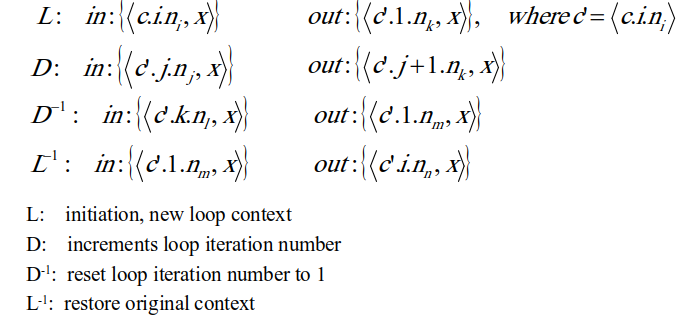
\includegraphics[width=\textwidth,height=8cm]{figures/dynamic_dataflow_interpreter.png}
    \end{center}
    \caption{U-interpreter for loop implementation.}
    \label{fig:dynamic_dataflow_interpreter}
  \end{small}
\end{figure}

\begin{figure}[htb]
  \begin{small}
    \begin{center}
      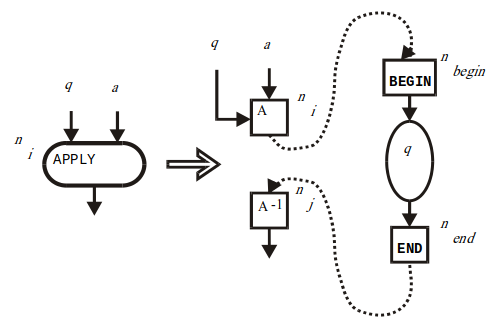
\includegraphics[width=\textwidth,height=8cm]{figures/dynamic_dataflow_interpreter_call.png}
    \end{center}
    \caption{U-interpreter for procedure calls.}
    \label{fig:dynamic_dataflow_interpreter_call}
  \end{small}
\end{figure}

Explicit token store dataflow model~\cite{DBLP:conf/isca/PapadopoulosC90}
has the target for efficient implementation of token matching,
as figure~\ref{fig:explicit_token_store_dataflow} showed.
It allocates a separate frame in the frame memory for each active loop iteration or subprogram invocation.
A frame consists of slots where each slot holds an operand that is used in the corresponding activity. 
Since access to slots is direct (i.e. through offsets relative to the frame pointer), no associative search is needed.

\begin{figure}[htb]
  \begin{small}
    \begin{center}
      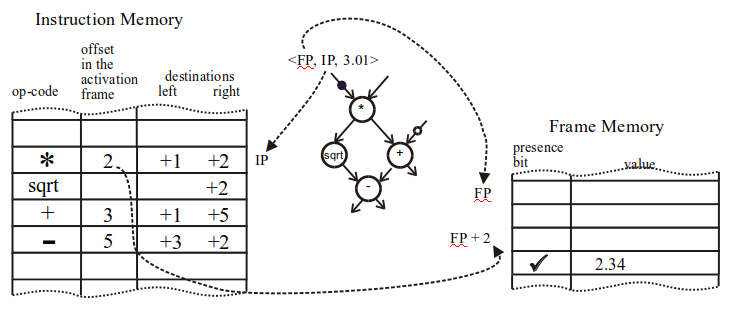
\includegraphics[width=\textwidth,height=8cm]{figures/explicit_token_store_dataflow.png}
    \end{center}
    \caption{Explicit token store dataflow with frame memory.}
    \label{fig:explicit_token_store_dataflow}
  \end{small}
\end{figure}

Dynamic dataflow has better performance (compared with static)
as it allows multiple tokens on each arc thereby unfolding more parallelism. 
But it needs a efficient implementation of the matching unit that collects tokens with matching tags
(Unfortunately, it is not cost-effective since the amount of memory needed to store tokens waiting for a match tends to be very large. 
As a result, all existing machines use some form of hashing techniques that are typically not as fast as associative memory).
And it has a bad single thread performance and poor sequential code performance (when not enough workload is present),
dyadic instructions lead to pipeline bubbles when first operand tokens arrive,
it has no instruction locality.

Large-Grain (coarse-grain) dataflow node contains a sequential block of instructions.
A macro dataflow node is activated in the dataflow manner, 
its instruction sequences is executed in the von Neumann style.
Off-the-shelf microprocessors can be used to support the execution stage. 
Large-grain dataflow machines typically decouple the matching stage
(sometimes called signal stage, synchronization stage, etc.)
from the execution stage by use of FIFO-buffers. 
Pipeline bubbles are avoided by the decoupling and FIFO-buffering. 

\subsection{Out of Order Execution}
Active/Instruction window size
(determined by both scheduling window and reorder buffer size)
limits the latency tolerance scalability of Tomasulo's algorithm.
A out-of-order engine dynamically builds the dataflow graph of a piece of the program.

Dataflow at the ISA level has not been successful,
dataflow implementations under the hood have been very successful (e.g OoO execution).

\clearpage

\section{Pure Dtaflow Architecture}
Treleaven had a survey of dataflow architecture~\cite{DBLP:journals/csur/TreleavenBH82}.
Data flow is based on a by-value data mechanism
and a parallel control mechanism, supported by data tokens. 

Dennis~\cite{DBLP:conf/isca/DennisM74} proposed ``The Elementary Processor'',
as figure~\ref{fig:elementory_processor}.
When a Cell contains an instruction and the necessary operands,
it is enabled and signals the Arbitration Network
that it is ready to transmit its contents as an operationace
to an Operation Unit which can perform the desired function.
The result of an operation leaves an Operation Unit
as one or more data packet,
consisting of the computed value and the address of a register
in the Memory to which the value is to be delivered.
The Distribution Network accepts data packets
from the Operation Units and utilizes the address of each
to direct the data item through the network to the correct register in the Memory.
The Instruction Cell containing that register may then be enabled
if an instruction and all operands are present in the Cell.

\begin{figure}[htb]
  \begin{small}
    \begin{center}
      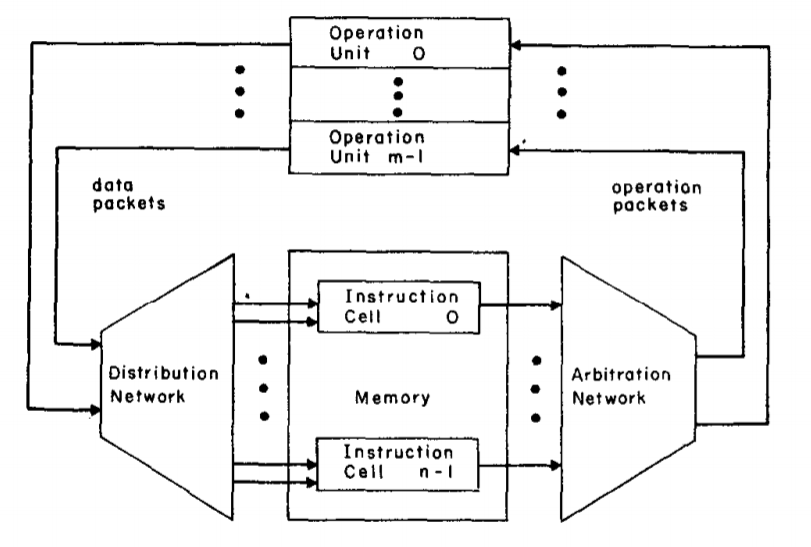
\includegraphics[width=\textwidth,height=8cm]{figures/isca94_elementory_processor.png}
    \end{center}
    \caption{ISCA94 - Elementary processor.}
    \label{fig:elementory_processor}
  \end{small}
\end{figure}

The Manchester prototype dataflow computer~\cite{DBLP:journals/cacm/GurdKW85} proposed
a powerful dataflow processing engine based on dynamic tagging.
Instructions do not reference memory, since the data-dependence arcs
allow data to be transmitted directly from generating instruction to subsequent instruction.
Consequently, instructions can be viewed as \textbf{pure operations}.
Individual systems differ mainly in the way they handle re-entrant code.
Static systems do not permit concurrent reactivation,
and so they are restricted to implementing loops and cannot accommodate recursion.
Dynamic systems permit recursive reactivation,
either by code-copying or tagging, at every occurrence of re-entry.

The MIT tagged-token architecture~\cite{DBLP:journals/tc/ArvindN90} proposed
a novel multiprocessor dataflow architecture.
A traditional von Neumann processor has fundamental characteristics
that reduce its effectiveness in a parallel machine:
\begin{compactitem}
  \item its performance suffers in the presence of long memory and communication latencies;
  \item they do not provide good synchronization mechanisms
        for frequent task switching between parallel activities;
  \item it is a significant added complication for the programmer to manage parallelism explicitly.
\end{compactitem}
A token carries the address of an instruction in this fixed code,
and a dynamic context that specifies the frame for a particular invocation of the function.
The format of a token can now be seen: $(c, s, v)_p$.
Here, $c$ is the context, $s$ is the address of the destination instruction, $v$ is the datum,
and $p$ is the port identifying which input of the instruction this token is meant for.
The value $(c, s)$ is called the fag of the token.

Monsoon~\cite{DBLP:conf/isca/PapadopoulosC90} is an explicit token store machine,
each PE is using an eight-stage pipeline:

\begin{compactitem}
  \item instruction fetch: precedes token matching (in contrast to dynamic dataflow processors with associative matching units),
  \item effective address generation: explicit token address is computed from the frame address and operand offset,
  \item presence bit operation: a presence bit is accessed to find out if the first operand of a dyadic operation has already arrived,
        if not arrived, presence bit set and the current token is stored into the frame slot of the frame memory,
        if arrived, presence bit is reset and the operand can be retrieved from the slot of the frame memory in next stage,
  \item frame operation stage: operand storing or retrieving,
  \item next three stages: execution stages in the course of which the next tag is also computed concurrently,
  \item form-token: forms one or two new tokens that are sent to the network, stored in a user token queue,
        a system token queue, or directly recirculated to the instruction fetch stage of the pipeline.
\end{compactitem}

\clearpage

\section{Raw Machine}

RAW~\cite{DBLP:conf/asplos/LeeBFSBSA98} use static orchestration to manage global operations,
but in a dynamically scheduled.

\clearpage

\section{TRIPS Architecture}

TRIPS architecture~\cite{DBLP:conf/isca/SankaralingamNLKHBKM03} proposed 
a polymorphous dataflow processor using static loop execution model.

Specialized architecture design led to performance fragility,
in which applications incur large swings in performance
based on how well they map to a given design.
One strategy for combating processor fragility is to build a heterogeneous chip multiprocessor (diverse cores).
An alternative approach (easier) is to use multiple heterogeneous processors.
This architectural ``polymorphism'' can defined as the capability to \textbf{configure hardware}
for \textbf{efficient execution} across broad classes of applications.

A key question, is what granularity of processors and memories
on a \textbf{CMP} is best for polymorphous capabilities.
The finer-grained architectures (e.g FPGAs) can offer high performance
on applications with fine-grained (data) parallelism,
but will have difficulty achieving good performance on general-purpose and serial applications.
A synthesis appraoch uses a fine-grained CMP to exploit regular, fine-grained parallelism
and tackles irregular, corse-grained parallelism by
synthesizing multiple processing elements (PEs) into larger ``logical'' processors.

The key challenge in defining the polymorphous features
is balancing their appropriate granularity so that
workloads involving different levels of ILP, TLP and DLP
can maximize their use of the available resources,
and at the same time avoid escalating complexity and nonscalable structures.

\subsection{EDGE ISA}

EDGE ISA~\cite{DBLP:journals/computer/BurgerKMDJLMBMY04} proposed:

\begin{compactitem}
  \item fine-grained concurrency with pipeline depth limits
  \item power-efficient high performance with hastened power limits
  \item on-chip communication-dominated execution (direct instruction communication)
  \item polymorphous execution and memory units in different modes
\end{compactitem}

Out-of-order issue RISC and CISC designs require many inefficient and power-hungry structures,
such as per-instruction register renaming (direct temporary value from producer to consumer),
associative issue window searches (64 instruction buffers per node),
complex dynamic schedulers,
high-bandwidth branch predictors (only needs to predict a branch once every 8 (128 instructions per node / 16 node per core) cycles),
large multiported register files (direct temporary value from producer to consumer),
and complex bypass networks (a simple point-to-point routing network with the average distance is short
because the compiler places dependent instructions on the same node or on nearby nodes).
In an EDGE architecture, a producer with multiple consumers would specify each of those consumers explicitly,
rather than writing to a single register that multiple consumers read (RISC architecture).
The ISA directly expresses the dataflow graph that the compiler generates internally,
instead of requiring the hardware to rediscover data dependences dynamically at runtime (RISC/CISC architectures).

An EDGE compiler has two new responsibilities in addition to those of a classic optimizing RISC compiler.
The first is forming large blocks (hyperblocks in the TRIPS architecture) that have no internal control flow,
thus permitting them to be scheduled as a unit.
The second is the spatial scheduling of those blocks,
in which the compiler statically assigns instructions in a block to ALUs in the execution array,
with the goal of reducing interinstruction communication distances and exposing parallelism.
RISC relies too little on the compiler, while VLIW relies on it too much. 
EDGE ISA provide a proper division between the compiler and architecture,
matching their responsibilities to their intrinsic capabilities,
and making the job of each simpler and more efficient.
A typical TRIPS code example is as figure~\ref{fig:trips_code}.

\begin{figure}[htb]
  \begin{small}
    \begin{center}
      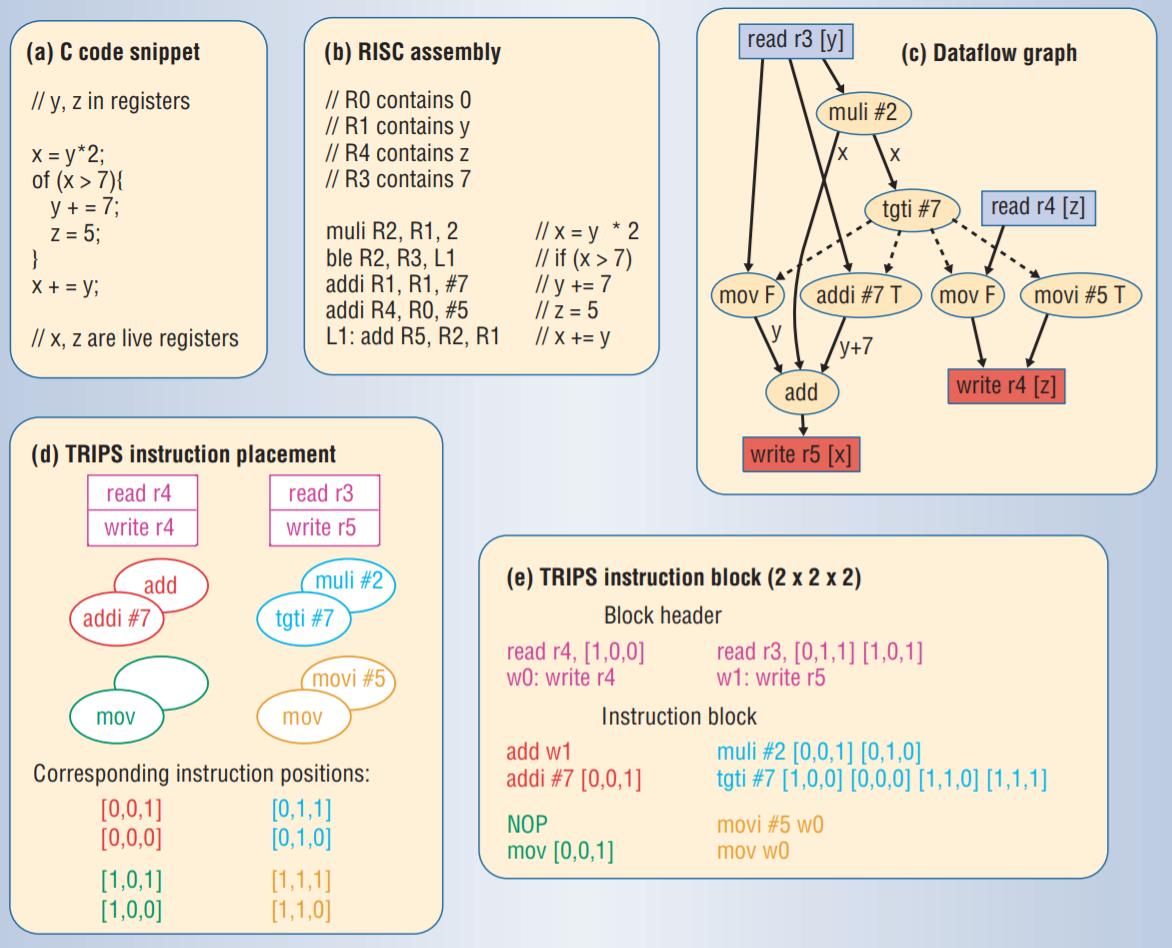
\includegraphics[width=\textwidth,height=10cm]{figures/ieee_computer_trips_code.png}
    \end{center}
    \caption{TRIPS code example.}
    \label{fig:trips_code}
  \end{small}
\end{figure}

\subsection{Core Execution Model}
The TRIPS architecture is fundamentally \emph{block oriented}.
Programs compiled for TRIPS are partitioned into large blocks of instructions
with a single entry point, no internal loops (and possibly multiple exit points).
Each block has a static set of state inputs,
and a potentially variable set of state outputs
that depends upon the exit point from the block.
At runtime, the basic operational flow of the processor includes fetching a block from memory,
loading it into the computational engine, executing it to completion,
committing its results to the persistent architectural state if necessary,
and then proceeding to the next block.
The TRIPS microarchitecture behaves like a conventional processor with sequential semantics at the block level,
with each block behaving as a ``megainstruction''.
The compiler builds 128-instruction blocks,
organized into groups of eight instructions per node at each of the 16 execution nodes.
Branches can only jump out of a hyperblock to the start of another hyperblock,
never to another point in the same hyperblock or into the middle of another.

\subsection{Architecture Overview}
The TRIPS prototype chip will consist of four polymorphous 16-wide cores,
an array of 32KB memory tiles connected by a routed network,
and a set of distributed memory controllers with channels to external memory,
as figure~\ref{fig:trips_arch}.

\begin{figure}[htb]
  \begin{small}
    \begin{center}
      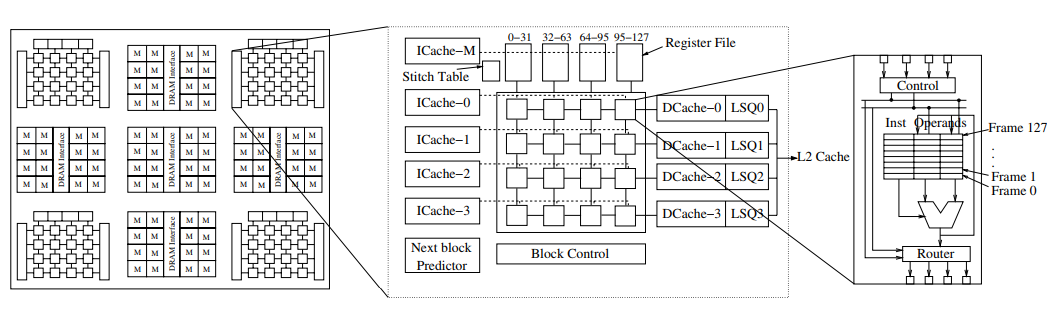
\includegraphics[width=\textwidth,height=5cm]{figures/isca03_trips_arch.png}
    \end{center}
    \caption{ISCA03 - TRIPS architecture.}
    \label{fig:trips_arch}
  \end{small}
\end{figure}

A TRIPS core is typically composed of an array of homogeneous execution nodes,
each containing an integer ALU, a floating point unit, a set of reservation stations
(store for an insturction and two source operands, 64 instruction buffers,
TRIPS microarchitecture supports up to 8 blocks (16 * 64 / 128 = 8) executing concurrently,
128 instructions per block, 16 * 64 = 1024 instruction buffers per core),
and router connections at the input and output.
The nodes are directly connected to their nearest neighbors,
but the routing network can deliver results to any node in the array.
Instruction cache for each row, L1 Data cache for every ALU (through the local grid rounting network).
The block control logic that is responsible for sequencing block execution and selecting the next block.
The partitioned register file requires fewer ports because the processor never
writes temporary values produced and consumed within a block to the register file.

\subsection{The TRIPS Resources}
The TRIPS architecture contains three main types of resources: 
the hardcoded, non-polymorphous resources for all modes (opreate in the same manner),
polymorphous resources for all modes (but can be configured to operate differently),
the resources that are not required for all modes.Frame space, register file banks,
block sequencing controls and memory tiles are polymorphous resources.
Reservation stations with the same index \textbf{across all of the nodes} combine to form a physical frame,
the frame space, or collection of frames, is a polymorphous resource in TRIPS.

\subsection{D-morph: Instruction-Level Parallelism}
The desktop morph, or D-morph, of the TRIPS processor
uses the polymorphous capabilities of the processor
to run \textbf{single-threaded} codes efficiently by exploiting
instruction-level parallelism.
To achieve high ILP, the D-morph configuration treats
the instruction buffers as a large, distributed, instruction issue window.
The D-morph must provide high-bandwidth instruction fetching,
aggressive control and data speculation, and a high-bandwidth, low-latency memory system.

The instruction issue window is fundamentally a three-dimensional scheduling region,
where the x- and y-dimensions correspond to the physical dimensions of the ALU array
and the z-dimension corresponds to multiple instruction slots at each ALU node.
A 3-D region (the array and the set of frames) into
which one hyperblock is mapped is called an architectural frame, or A-frame.
Consumers are encoded in the producer instructions as X, Y, and Zrelative offsets.
Each producer instruction prepends its A-frame ID to the Z-coordinate of its consumer to
form the correct instruction buffer address of the consumer.
Values passed between hyperblocks are transmitted through
the register file using the register stitch table.

To summarize, with accurate exit prediction, high-bandwidth I-fetching,
partitioned data caches, and concurrent execution of hyperblocks with inter-block value forwarding,
the D-morph is able to use the instruction buffers as a polymorphous out-of-order issue window effectively.

\subsection{T-morph: Thread-Level Parallelism}
Frame processors time-share the processor by allocating threads to unique sets of physical frames.
a TRIPS core can dedicate all 128 frames to a single thread in the Dmorph,
or 64 frames to each of two threads in the T-morph (uneven frame sharing is also possible).
The T-morph maintains n program counters (where n is the number of concurrent threads allowed)
and n global history shift registers in the exit predictor to reduce thread-induced mispredictions.
Per-thread IDs on cache tags are necessary to prevent illegal cross-thread interference.

\subsection{S-morph: Data-Level Parallelism}
Streaming media and scientific applications are characterized by data level parallelism (DLP)
including predictable loop-based control flow with large iteration counts,
large data sets, regular access patterns, poor locality but tolerance to memory latency,
and high computation intensity with tens to hundreds of arithmetic operations performed per element loaded from memory.

The S-morph fuses multiple A-frames to make a super A-frame,
instead of using separate A-frames for speculation or multithreading.
Inner loops of a streaming application are unrolled
to fill the reservation stations within these super A-frames.
The S-morph employs mapping reuse, in which a block is kept in the reservation stations and used multiple times
Until the iteration counter reaches zero, the super A-frame is cleared
and the hardware maps the next block onto the ALUs for execution.

\clearpage

\section{WaveScalar Architecture}
WaveScalar ~\cite{DBLP:conf/micro/SwansonMSO03}\cite{DBLP:journals/tocs/SwansonSMPPMOE07}
is a dataflow instruction set architecture and execution model designed for scalable,
low-complexity/high-performance processors.
WaveScalar makes use of the implementation of loop in dynamic dataflow architecture.
WaveScalar architectures cache instructions and the value on in a \textbf{WaveCache},
a simple grid of ``alu-in-cache'' nodes.
By co-locating computation and data in physical space,
the WaveCache minimizes long wire, high-latency communication.

\subsection{Processor Scaling Wall}
Silicon technology will continue to provide an exponential increase in the availability of raw transistors.
However, effectively translating this resource into application performance is an open challenge
Simply scaling up current architectures will not convert these new transistors to commensurate increases in performance.

\begin{compactitem}
  \item fast transistors but slow wires;
  \item the increasing cost of circuit complexity;
  \item  the decreasing reliability of circuit technology (shrinking feature sizes
  and continued scaling of the underlying material characteristics)
\end{compactitem}
Due to slow broadcast networks, associative searches,
complex control logic, and inherently centralized structures,
modern superscalar processor designs will not scale easily.

\subsection{Key of WaveScalar}

Unlike past dataflow work focusing on maximizing processor utilization,
WaveScalar’s goal is to minimize communication costs by ridding the processor of long wires and broadcast networks.
It includes a completely \textbf{decentralized} implementation of the ``token-store'' of traditional dataflow architectures
and a \textbf{distributed} execution model.

WaveScalar efficiently supports traditional von Neumann-style memory semantics
in a dataflow model (\textbf{allow side effects}).
Such a memory ordering scheme can efficiently enables
true dataflow execution of programs written in \textit{any} language.

TRIPS~\cite{DBLP:conf/isca/SankaralingamNLKHBKM03}and Raw~\cite{DBLP:conf/asplos/LeeBFSBSA98},
have extended the von Neumann paradigm in novel ways,
but they still rely on a program counter (block counter)
to sequence program execution and memory access.
WaveScalar completely abandons the program counter and linear von Neumann execution.

WaveScalar instructions execute in-place in the memory system
and explicitly send their results to their dependents.
WaveScalar instructions are cached and executed
by an intelligent, distributed instruction cache – the WaveCache.
The WaveCache loads instructions from memory and assigns them to processing elements for execution.
Optimizing instruction placement allows a WaveCache to
take advantage of predictability in the dynamic data dependencies of a program,
which called \textit{dataflow locality}.

\clearpage

\section{Dataflow for AI}

ASIC- or FPGA-based AI-EI chips often use a spatial architecture.
Compared to general-purpose chips, dedicated chips are used
in specific scenarios and their functions are limited.
A simple and regular hardware architecture is the basis for reducing design costs
and is a prerequisite for implementing low-cost dedicated chips.
A low enough chip cost can hedge the limitations of dedicated chip functionality.

The spatial architecture uses Dataflow processing.
In the spatial architecture, the ALU forms a data processing chain
that enables data to be transferred directly between ALUs.
In this spatial architecture, each ALU has its own control logic and local storage (register file).
Among them, the ALU with local storage is defined as PE.

For spatial architectures, hardware design is based on
low-energy memory in hierarchical memory and increases data reuse
(essentially, convolution is spatial reuse, which reuses spatial invariance) to reduce power consumption.
In addition, Dataflow controls data reading, writing, and processing.
In general, the spatial architecture balances I/O and computational problems
based on hierarchical memory and data flow,
thereby reducing power consumption and increasing computational throughput.

In the inference of deep learning, there are a large number of computational requirements.
However, these calculations are performed in a hierarchical order.
Therefore, the control process is relatively simple and clear.
It can be seen that the Dataflow processing method is very consistent
with the computational requirements based on the deep neural network inference part.

The data stream can determine which data is read into which memory and when it is processed.
In addition, there is no randomness in DNN inference.
Therefore, an AI-EI chip based on the fixed architecture of Dataflow
can be designed from the perspective of optimal power consumption.
Currently, most AI-EI chips for deep learning inference use Dataflow.

In hierarchical memory, a large amount of memory read and write operations
consumes much more energy than a small memory.
Thus, once a piece of data has been moved from large memory to small memory,
the data block is reused as much as possible to minimize power consumption.
However, low-power memory has limited storage space.
How to maximize the reuse rate is the most important condition
for designing based on the Dataflow accelerator.
That is, by maximizing the data reuse rate to reduce I/O requirements
and reduce data processing power consumption,
thereby increasing throughput and reducing overall energy consumption.
Common DNN data stream types include: weight fixed data stream, output fixed data stream, No local reuse (NLR), and row fixed data stream.

Weighted fixed data stream: The weight data is read from the DRAM,
placed in the RF of the PE and remains unchanged,
then the input data is broadcasted to each PE,
and finally the part and (partialsum) of the PE array are obtained.
The processing method reduces the number of times the weight data is read from the RF of the PE,
and minimizes the number of times the weight is directly read from the DRAM,
thereby maximizing the multiplexing rate of the convolution
and the weight of the filter to reduce the multiplexing rate and energy consumption.
NeuFlow is an AI-EI chip based on this type of data processing.

Output fixed (OS) data stream: By inputting data in the stream in the PE array
and then broadcasting the weight data to the PE array,
the sum of the parts in the RF is kept constant,
thereby minimizing the energy consumption of the read and write parts.
The Cambrian ShiDianNao is based on an output fixed AI-EI chip.
In addition, depending on the processing target,
the data stream can be divided into OS\_A with the convolution layer as the processing target
and OS\_C with the full connection layer as the processing target.
OS\_B is an OS data stream between OS\_A and OS\_C.

NLR data stream: The RF of the PE array does not store any fixed data.
On the contrary, in this case, all data read and write operations are performed in the global buffer.
The Cambrian DianNao and DaNiaoNao are AI-EI chips based on this data processing method.

Fixed data stream: Maximize all data multiplexing rates and make all data read and write operations in RF as much as possible,
reducing read and write operations on global buffers to reduce power consumption.
Each PE can complete a 1D convolution operation,
and multiple PEs can perform a 2D convolution operation.
In a two-dimensional PE array, the weight data of each row is multiplexed on the PE unit on the horizontal axis,
and the input data of each row is multiplexed on the PE unit on the diagonal line,
and multiple on the vertical axis On the PE unit,
the portion of each row and the data are multiplexed, that is,
the fixed data stream can maximize the multiplexing rate of all data,
thereby optimizing the power consumption globally.
Eyeriss' NPU is based on line-fixed AI-EI chips.

\clearpage

\bibliographystyle{unsrt}
\bibliography{bibs/dataflow}
\addcontentsline{toc}{section}{References}
\newpage

\end{document}
